\documentclass[12pt]{article}
\usepackage[utf8]{inputenc} % Obsługa kodowania utf8
\usepackage[T1]{fontenc} % Obsługa polskich znaków w fontach
\usepackage{graphicx} % Required for inserting images
\usepackage{float} 
\usepackage{geometry}
\usepackage{ragged2e}
\usepackage{listings}
\usepackage{xcolor}
\usepackage{caption} 


\captionsetup[figure]{name=Rys.}

% Ustawienia dla kolorów
\definecolor{codegreen}{rgb}{0,0.6,0}
\definecolor{codegray}{rgb}{0.5,0.5,0.5}
\definecolor{codepurple}{rgb}{0.58,0,0.82}
\definecolor{backcolour}{rgb}{1.0,1.0,1.0}

% Ustawienia dla wyglądu kodu
\lstdefinestyle{mystyle}{
    backgroundcolor=\color{backcolour},   
    commentstyle=\color{codegreen},
    keywordstyle=\color{blue},
    numberstyle=\tiny\color{codegray},
    stringstyle=\color{codepurple},
    basicstyle=\footnotesize,
    breakatwhitespace=false,         
    breaklines=true,                 
    captionpos=b,                    
    keepspaces=true,                 
    numbers=left,                    
    numbersep=5pt,                  
    showspaces=false,                
    showstringspaces=false,
    showtabs=false,                  
    tabsize=2
}

\lstset{style=mystyle}


\geometry{
    top=2cm,
    bottom=2cm,
    left=1cm,
    right=1cm
}


\graphicspath{{images/}}
\title{Projekt \par Bezzałogowe Obiekty Autonomiczne  \par \vspace{10pt} \textbf{Symulacja robota Unitree Go2 w środowisku ISSAC SIM}}
\date{}  




\begin{document}
\begin{figure}[t]
\centering
    
\includegraphics[width=0.8\textwidth]{Zdjęcia/Polsl.png}
\end{figure}

\maketitle
\vspace{150pt}
Skład sekcji: Filip Bazarnicki, Darian Bonk, Jakub Ligenza, Kacper Wach

Rok akademicki: 2024/25


Kierunek: Automatyka i Robotyka

Specjalizacja: Robotyka

Semestr: 1


\newpage

\section{Cel projektu}

Celem projektu była instalacja środowiska ISSAC SIM oraz jego odpowiednia konfiguracja, przygotowanie cyfrowego bliźniaka robota Unitree Go2 przeprowadzenie przykładowych symulacji w ISAAC SIM oraz nawiązanie połączenia między nim, a środowiskiem ROS2.

\section{Instalacja i konfiguracja środowiska ISSAC SIM oraz ROS2}

\section{Cyfrowy bliźniak robota Unitree Go2}

W środowisku ISSAC SIM znajduję się gotowy model cyfrowego bliźniaka robota Unitree Go2, w celu umieszczenia go na scenie otwartego programu należy odnaleźć go w oknie Isaac Sim Assets i dodać go wciskając przycisk Load as Reference lub przeciągając jego ikonę na scenę, widok okna Isaac Sim Assets przedstawiony jest na rysunku \ref{fig:Assets}. Widok umieszczonego w symulacji robota przedstawiony jest na rysunku \ref{fig:cyfrowyBlizniak}.  

\begin{figure}[h]
    \centering
    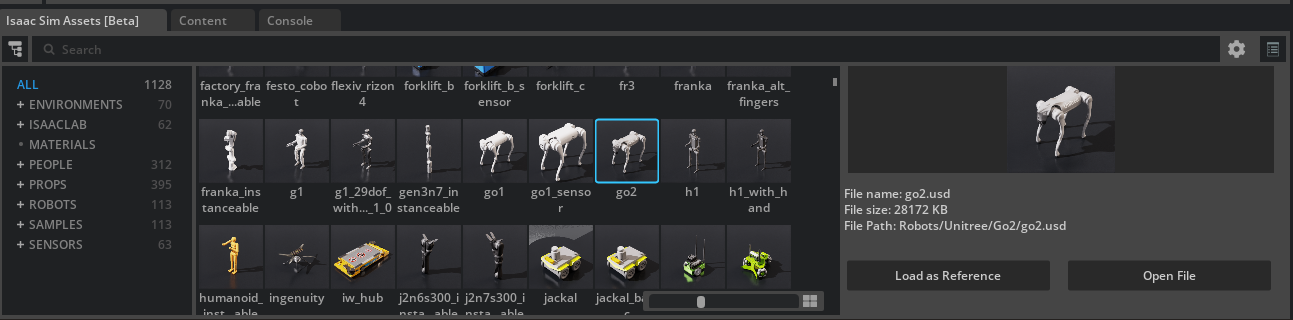
\includegraphics[width=0.75\linewidth]{bibliotekaAssets.png}
    \caption{Biblioteka dostępnych robotów Isaac Sim Assets.}
    \label{fig:Assets}
\end{figure}

\begin{figure}[h]
    \centering
    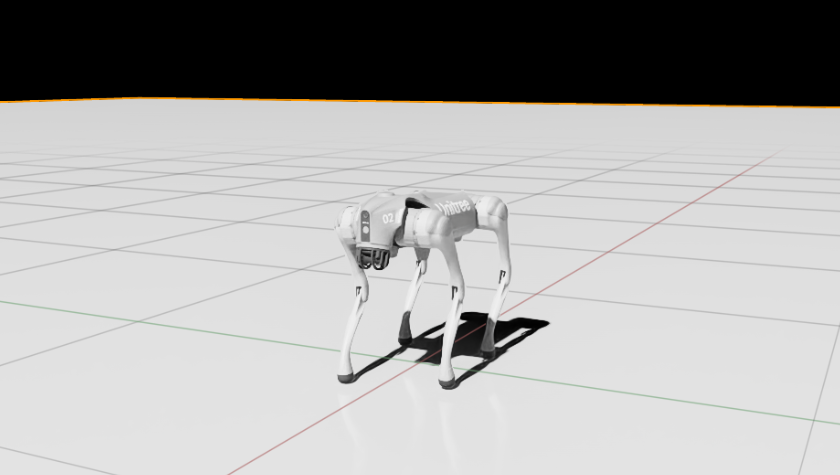
\includegraphics[width=0.5\linewidth]{Zdjęcia/cyfrowyBlizniakUnitryGo2.png}
    \caption{Cyfrowy bliźniak robot Unitree Go2 w środowisku ISAAC SIM.}
    \label{fig:cyfrowyBlizniak}
\end{figure}

\section{Sterowania robotem środowiskiem ROS2}
\begin{figure}[h]
    \centering
    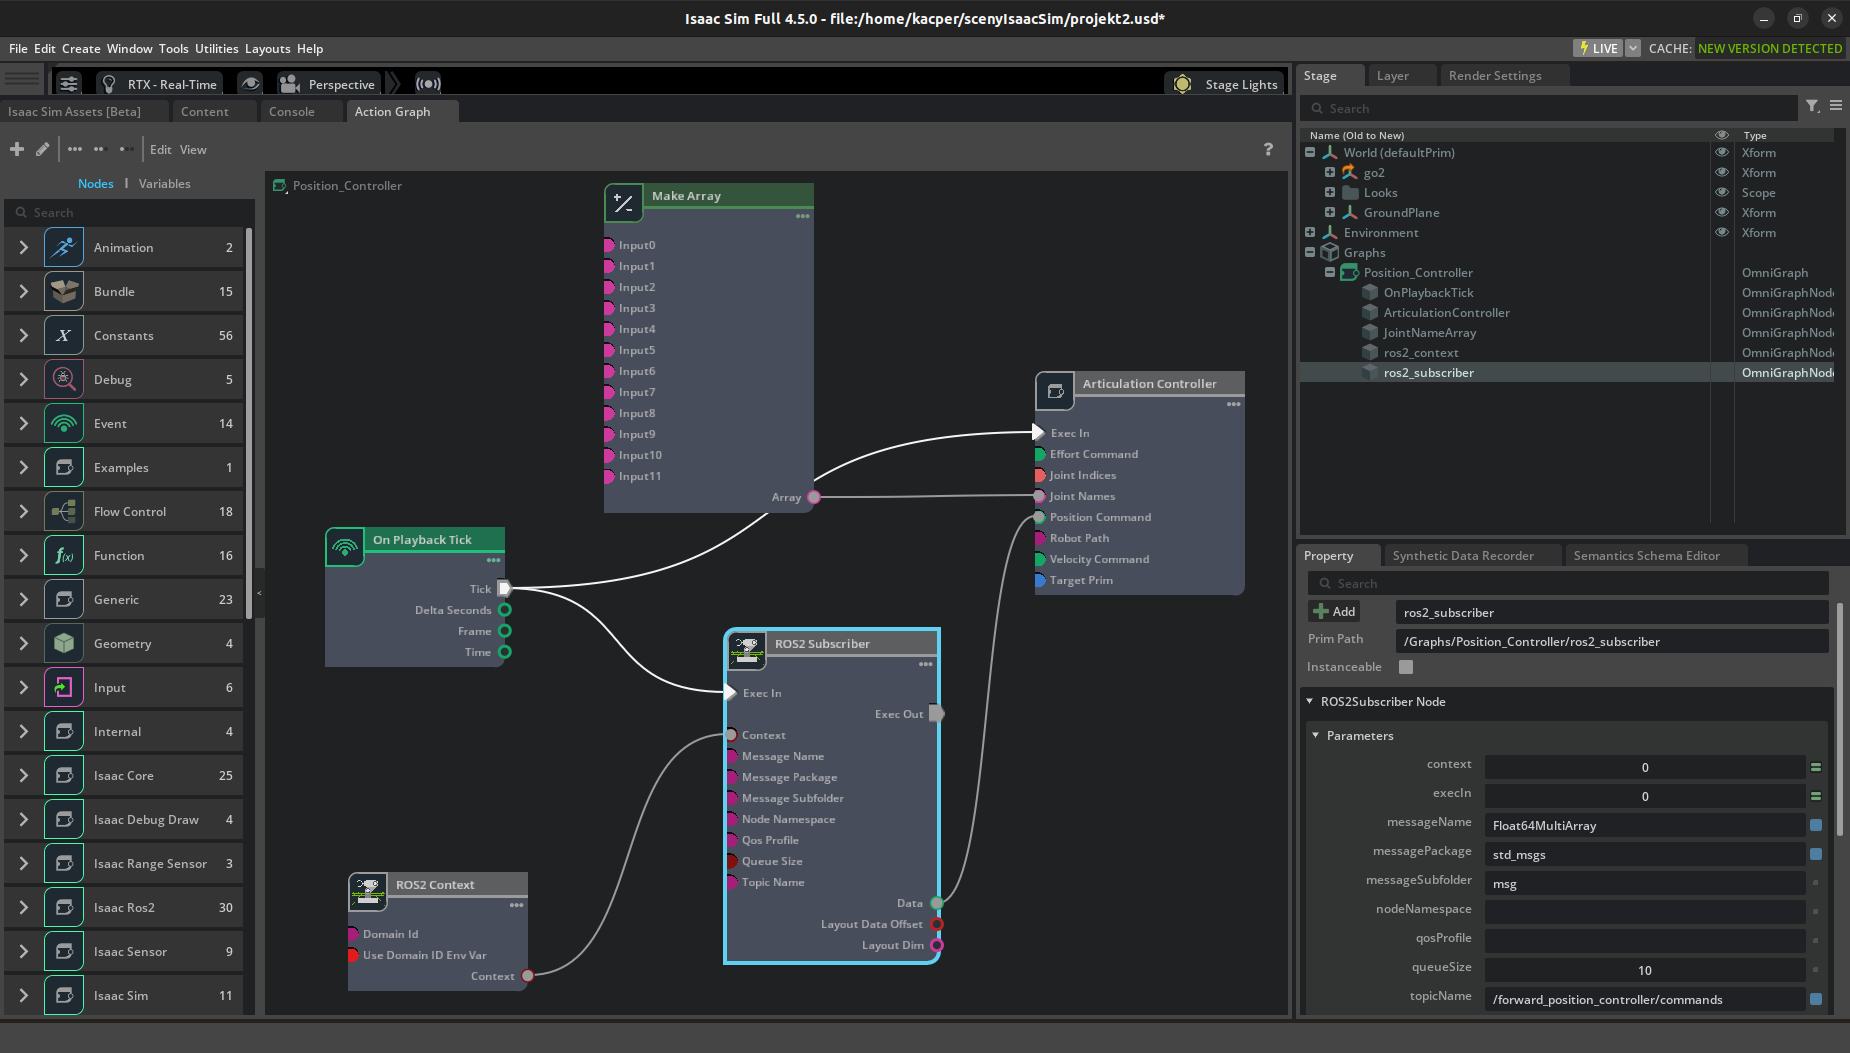
\includegraphics[width=0.75\linewidth]{Zdjęcia/actionGraph.png}
    \caption{Action Graph do nawiązania komunikacji między ROS2 oraz ISAAC SIM.}
    \label{fig:actionGraph}
\end{figure}

\begin{figure}[h]
    \centering
    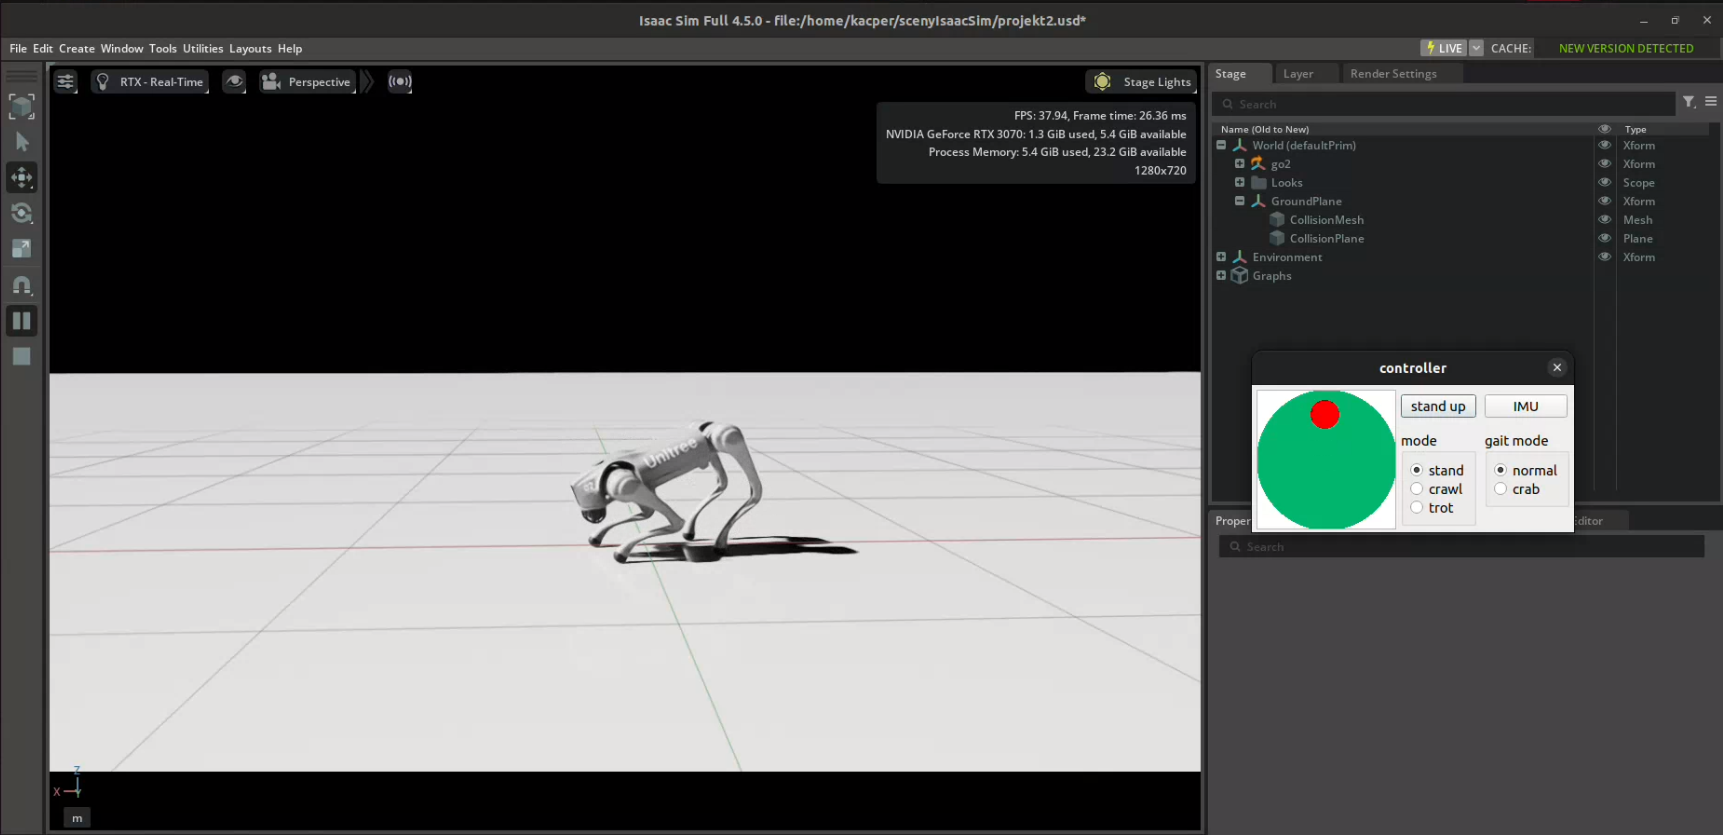
\includegraphics[width=0.75\linewidth]{Zdjęcia/pochyleniePrzod.png}
    \caption{Robot Unitree Go2 pochylający się do przodu.}
    \label{fig:pochyleniePrzod}
\end{figure}

\begin{figure}[h]
    \centering
    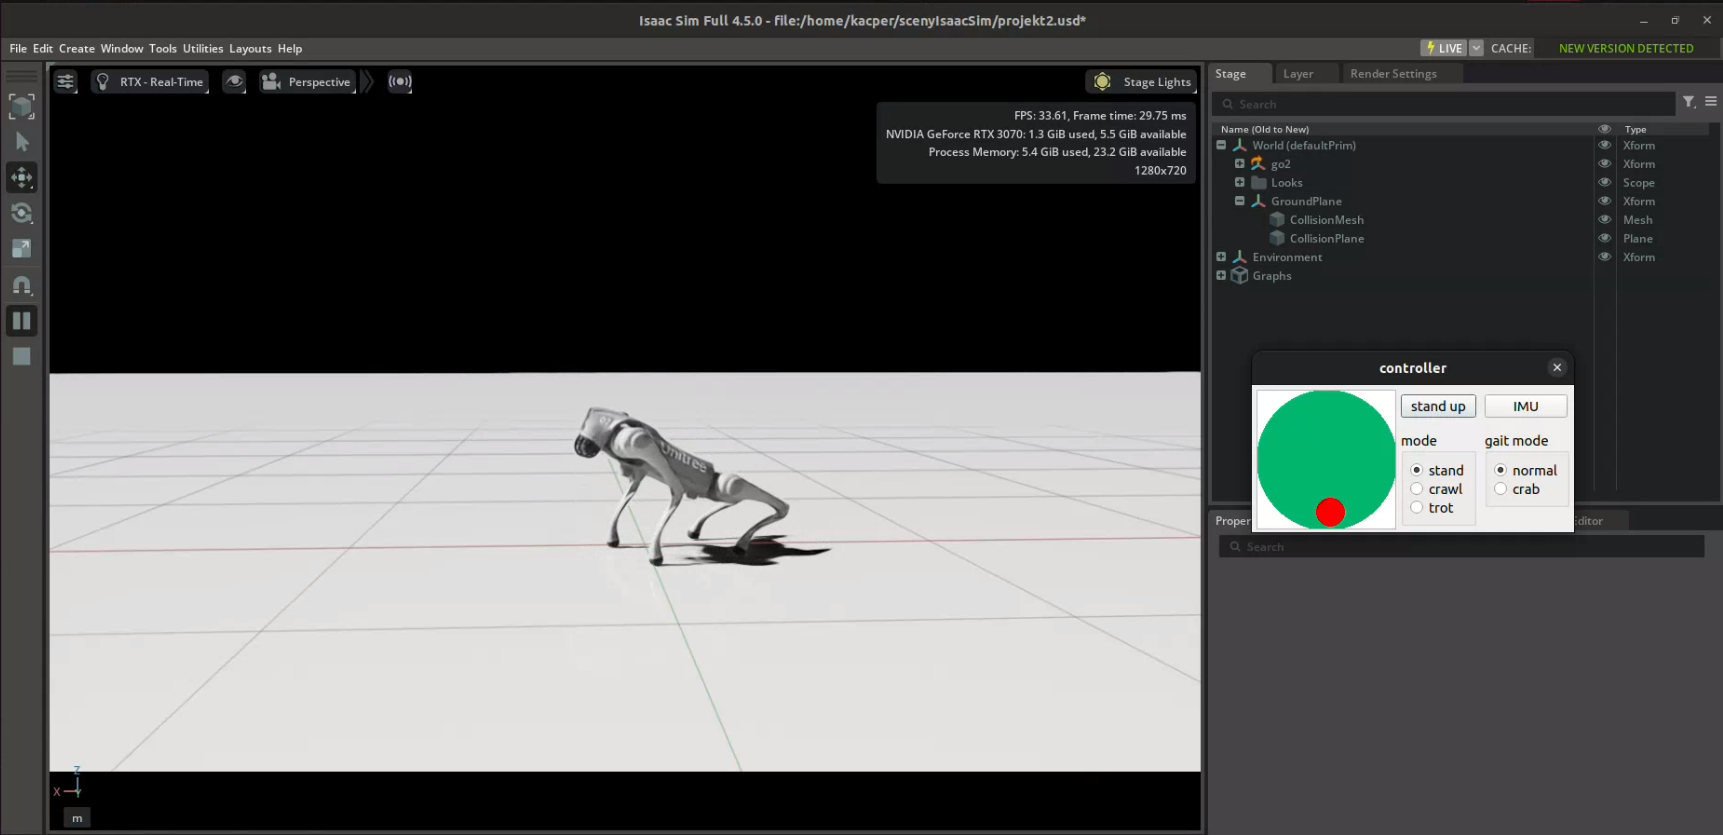
\includegraphics[width=0.75\linewidth]{Zdjęcia/pochylenieTyl.png}
    \caption{Robot Unitree Go2 pochylający się do tyłu.}
    \label{fig:pochylenieTyl}
\end{figure}

\section{Przykładowe symulacje}

\end{document}
